\documentclass[aspectratio=169]{beamer}
\usetheme{Copenhagen}
%% Remove draft for real article, put twocolumn for two columns
\usetheme{metropolis}
\usepackage{multicol}
\usepackage[style=british]{csquotes}

\def\signed #1{{\leavevmode\unskip\nobreak\hfil\penalty50\hskip1em
  \hbox{}\nobreak\hfill #1%
  \parfillskip=0pt \finalhyphendemerits=0 \endgraf}}

\newsavebox\mybox
\newenvironment{aquote}[1]
  {\savebox\mybox{#1}\begin{quote}\openautoquote\hspace*{-.7ex}}
  {\unskip\closeautoquote\vspace*{1mm}\signed{\usebox\mybox}\end{quote}}

\usepackage[utf8]{inputenc}
\newtheorem*{question}{Question}

\newcommand{\vectorproj}[2][]{\mathrm{proj}_{\vect{#1}}\vect{#2}}
\newcommand{\vectorcomp}[2][]{\mathrm{comp}_{\vect{#1}}\vect{#2}}
\newcommand{\vect}{\mathbf}
\newcommand{\R}{\mathbb{R}}
%% commentary bubble
\newcommand{\SV}[2][]{\sidenote[colback=green!10]{\textbf{SV\xspace #1:} #2}}

\title{ Multivariable Calculus \\ Day  20 \\ Vector Calculus: Line integrals}
\date{Spring 2023}

\begin{document}

\maketitle

\begin{frame}
    \frametitle{ Warning}
    Don't be confused with arc length!!!
\end{frame}

\begin{frame}
    \frametitle{Line integrals}
    \begin{definition}
        Let $D$ be a domain on $\R^n$.
        A vector field on $\R^n$ is a function $\vect{F}: D \to \R^n$
        that assign each point $\vect{x}\in D$ to a vector $\vect{F}(\vect{x}) \in \R^n$.
    \end{definition}
    We only think about vector fields on $\R^2$ and $\R^3$.

    \pause

    In \(\mathbb{R}^2\), one typically write the vector fields in terms of \textbf{component functions} \(P, Q\)
\[\mathbf{F}(x,y) = P(x,y) \mathbf{i} + Q(x,y) \mathbf{j}\,.\]

    
In \(\mathbb{R}^3\), one typically write the vector fields in terms of \textbf{component functions} \(P, Q, R\)
\[\mathbf{F}(x,y,z) = P(x,y) \mathbf{i} + Q(x,y) \mathbf{j} + R(x,y,z) \mathbf{k}\,.\]

\end{frame}

\begin{frame}
    \frametitle{Example}
    $$\vect{F}(x,y) = -y \vect{i} + x \vect{j} \,.$$
\end{frame}

\begin{frame}
    \frametitle{ Worksheet   }
    Matching the vector fields with the pictures

    $\vect{F}(x,y) = \langle x, - y \rangle$, 
    $\vect{F}(x,y) = \langle y, x- y \rangle$, 
    $\vect{F}(x,y) = \langle y, y + 2 \rangle$, 
    $\vect{F}(x,y) = \langle \cos(x+y), x \rangle$, 
    \begin{figure}
        \begin{center}
            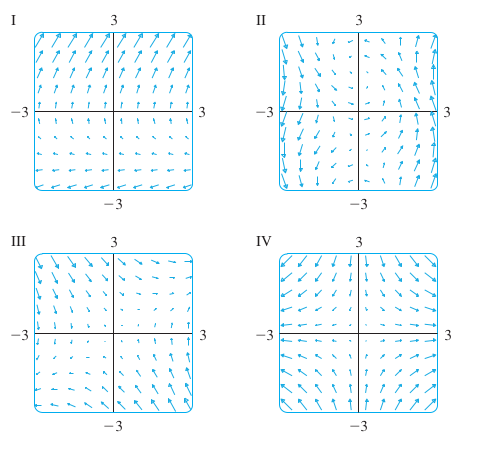
\includegraphics[width=0.4\textwidth]{vector-field.png}
        \end{center}
    \end{figure}
\end{frame}

\begin{frame}
    \frametitle{Line integrals}
    This is similar to integration of parametric curves but 
    there are differences.
\end{frame}

\begin{frame}
    \frametitle{Line integrals}
    We now perform a Riemann-sum-like action.
    \begin{definition}
    Let $C$ be a smooth curve.
    The \textbf{line integral of $f$ along $C$} is defined as
    \begin{equation*}
        \int_C f(x,y) \, ds = \lim_{n\to \infty} \sum_{i=1}^n f(x_i^*, y_i^*) \Delta s_i \,,
    \end{equation*}
    where $\Delta s_i$ is the length of a subarc of $C$.
    \end{definition}
\end{frame}

\begin{frame}
    \frametitle{Worksheet}
    Suppose the curve $C$ is given by the parametric equation
    \begin{equation*}
        \vect{r}(t) = \langle x(t), y(t) \rangle \,, \qquad t\in [a,b]\,.
    \end{equation*}
    Find a formula for 
    \begin{equation*}
        \int_C f(x,y) \, ds 
    \end{equation*}
    that can relate to the parametric equation.
    (Hint: use the arclength formula)
\end{frame}

\begin{frame}
    \frametitle{Example}
    \begin{enumerate}
        \item Evalutate
            \begin{equation*}
                \int_C (2 + x^2y) \, ds
            \end{equation*}
            where $C$ is the upper half of the unit circle.
        \item Evaluate 
            \begin{equation*}
                \int_C 2x \, ds
            \end{equation*}
            where $C$ consists of the arc $C_1$ of the parabola $y=x^2$ from
        $(0,0)$ to $(1,1)$ followed by the vertical line segment $C_2$ from $(1,1)$ to $(1,2)$.
    \end{enumerate}
\end{frame}

\end{document}

